\documentclass[11pt,a4paper,twoside,french,svgnames]{report}
\usepackage[utf8]{inputenc} % force the use of utf8
\usepackage[T1]{fontenc} % font encoding, allows accents
\usepackage[papersize={21cm,29.7cm},top= 2.5cm,bottom=2.5cm, inner=2.5cm, outer=2.5cm]{geometry} % page formatting
\usepackage[francais]{babel} % translate everything in the desired language: table of contents, etc. 'english' can be replaced with 'francais'
\usepackage{graphicx} % images management
\usepackage{wrapfig} % floating images
\usepackage{array} % allow arrays
\usepackage{fancyhdr} % headers/footers management (overrides empty, plain and headings)
\usepackage{listings} % code insertion (MUST BE WRITTEN AFTER BABEL)
%\usepackage[nottoc,numbib]{tocbibind} % bib in toc
%\usepackage{pdfpages} % include PDF documents
\usepackage{enumitem} % for /setlist
\usepackage{color,soul} % add some colors and hightlight
\usepackage{xcolor} % more colors
\usepackage[hyphens]{url} % auto break lines in URL
\usepackage{amsmath}
\usepackage[hidelinks,  colorlinks  = true, % no borders, colors enabled
                        anchorcolor = blue,
                        linkcolor   = black, % links in table of contents
                        urlcolor    = blue,
                        citecolor   = blue]{hyperref}
%\usepackage[%nonumberlist,% no page number
%            toc,% displayed in toc
%            numberedsection,% displayed as a numbered section in toc
%            xindy]{glossaries} % glossary with xindy style. MUST BE WRITTEN AFTER HYPERREF
%\setglossarystyle{listgroup}

\sethlcolor{cyan} % package soul
\newcommand{\file}[1]{\hl{\emph{#1}}} % highlight a file URI

%\makeglossaries
%\loadglsentries{glossary.tex}

%%%%%%%%%%%%%%%%%%%%%%%%%%%%%%%%%%%%%%%%%%%%%%%%%%%%%%%% LISTINGS %%%%%%%%%%%%%%%%%%%%%%%%%%%%%%%%%%%%%%%%%%%%%%%%%%%%%%%%
\definecolor{comment}{rgb}{0.12, 0.38, 0.18 } % adjusted, in Eclipse: {0.25, 0.42, 0.30 } = #3F6A4D
\definecolor{keyword}{rgb}{0.37, 0.08, 0.25}  % #5F1441
\definecolor{string}{rgb}{0.06, 0.10, 0.98} % #101AF9

\lstset{
  columns=flexible, %prevent extra spaces
  rulecolor=\color{black!50},
  backgroundcolor = \color{blue!10},
  numbers=none, % line numbering
  showspaces=false,
  showtabs=false,
  tabsize=4,
  breaklines=true,
  showstringspaces=false,
  breakatwhitespace=false,
  commentstyle=\color{comment},
  keywordstyle=\color{keyword},
  stringstyle=\color{string},
  basicstyle=\ttfamily,
  extendedchars=true,
  emph=[2]{In},
  emphstyle=[2]\color{black!70},
  morecomment=[l][\color{blue}]{Out},
  frame=single,
  frameround=tttt,
  framerule=0.3pt,
  framesep=4pt,
  belowcaptionskip=2.1pt,
  literate={à}{{\`a }}1 {â}{{\^a}}1 %                         letter a
           {À}{{\`A}}1 {Â}{{\^A}}1 %                         letter A
           {ç}{{\c{c}}}1 %                                   letter c
           {Ç}{{\c{C}}}1 %                                   letter C
           {é}{{\'e}}1 {è}{{\`e}}1 {ê}{{\^e}}1 {ë}{{\"e}}1 % letter e
           {É}{{\'E}}1 {È}{{\`E}}1 {Ê}{{\^E}}1 {Ë}{{\"E}}1 % letter E
           {î}{{\^i}}1 {ï}{{\"i}}1 %                         letter i
           {Î}{{\^I}}1 {Ï}{{\"I}}1 %                         letter I
           {ô}{{\^o}}1 %                                     letter o
           {Ô}{{\^O}}1 %                                     letter O
           {œ}{{\oe}}1 %                                     letter oe
           {Œ}{{\OE}}1 %                                     letter OE
           {ù}{{\`u}}1 {û}{{\^u}}1 {ü}{{\"u}}1 %             letter u
           {Ù}{{\`U}}1 {Û}{{\^U}}1 {Ü}{{\"U}}1 %             letter U
  % above is a hack to force UTF8 compatibility (only for french)
}

\newcommand{\textcode}[1]{\lstset{
  language=,
  title={{\setlength{\fboxsep}{1pt}\fcolorbox{orange}{yellow!20}{\sffamily\scriptsize
              \textcolor{gray!10}{\_}{#1}\textcolor{gray!10}{\_}}}}
  }
}

\newcommand{\assembly}{\lstset{
  language={[x86masm]Assembler},
  title={{\setlength{\fboxsep}{1pt}\fcolorbox{orange}{yellow!20}{\sffamily\scriptsize
              \textcolor{gray!10}{\_}Assembleur\textcolor{gray!10}{\_}}}}
  }
}
%%%%%%%%%%%%%%%%%%%%%%%%%%%%%%%%%%%%%%%%%%%%%%%%%%%%%%%%%%%%%%%%%%%%%%%%%%%%%%%%%%%%%%%%%%%%%%%%%%%%%%%%%%%%%%%%%%%%%%%%%%%

%\parindent=20pt
\fancypagestyle{plain}{
    % Headers
    \fancyhead[R]{Rapport TP7 MI01}
    \fancyhead[L]{Romain \textsc{PELLERIN} - Kyâne \textsc{PICHOU}}

    % Footers
    \renewcommand{\footrulewidth}{0.1pt}
    \fancyfoot[C]{Université de Technologie de Compiègne}
    \fancyfoot[LE]{\ifnum\thepage>0 \thepage \fi}
    \fancyfoot[RO]{\ifnum\thepage>0 \thepage \fi}
}

\fancypagestyle{empty}{%
    \renewcommand{\headrulewidth}{0pt} % No sub line
    \fancyhead{} % Empty the header

    \renewcommand{\footrulewidth}{0pt}
    \fancyfoot{}
} 

\setlist[itemize,2]{label={$\bullet$}} % use bullets for nested itemize

% First page
\newcommand{\presentation}[1]{\vspace{0.3cm}\large{\textbf{#1}}\vspace{0.3cm}\\}
\newcommand{\presentationLarge}[1]{\vspace{0.3cm}\LARGE{\textbf{#1}}\vspace{0.3cm}\\}

% Overrides chapter (numbered and no-numbered) headings: remove space, display only the title
\makeatletter
  \def\@makechapterhead#1{%
  \vspace*{0\p@}% avant 50
  {\parindent \z@ \raggedright \normalfont
    %\ifnum \c@secnumdepth >\m@ne
    %    \huge\bfseries \@chapapp\space \thechapter
    %    \par\nobreak
    %    \vskip 20\p@
    %\fi
    \interlinepenalty\@M
    \Huge \bfseries \thechapter\quad #1   
    \vskip 40\p@
  }}
  \def\@makeschapterhead#1{%
  \vspace*{0\p@}% before 50
  {\parindent \z@ \raggedright
    \normalfont
    \interlinepenalty\@M
    \Huge \bfseries  #1\par\nobreak
    \vskip 40\p@
  }}
\makeatother

\newcommand{\ignore}[1]{} % inline comments

\pagenumbering{arabic}
%\addtocounter{page}{-7} % page numbering starts at 1 + (-7)
\pagestyle{plain} % uses fancy

\title{Rapport MI01}
\author{Romain PELLERIN et Kyâne PICHOU}
\date\today

%\setcounter{tocdepth}{4}

\begin{document}
\thispagestyle{empty} % only for the current page

\begin{center}

\includegraphics[height=3cm]{UTC_logo.png}\\
\vspace{2.5cm}
\presentation{Université de Technologie de Compiègne} 
\presentation{MI01}

\vspace{2cm}
\noindent\fbox{
\begin{minipage}{0.9\textwidth}
\begin{center}
    \presentationLarge{Rapport de TP}
    \presentationLarge{\Huge{7 - Traitement d'image}}
\end{center}
\end{minipage}}
\vspace{3cm}

\presentation{Automne 2014}
\vspace{1cm}

\def\arraystretch{1.5} % 1 is the default
\begin{tabular}{|>{\hfill\arraybackslash}p{5cm}|p{5cm}|}
\hline
    \multicolumn{2}{|c|}{Romain \textsc{PELLERIN} - Kyâne \textsc{PICHOU}}\\
\hline
     \multicolumn{2}{|c|}{Groupe 1}\\% dates
\hline
    \multicolumn{2}{|c|}{\textit{\today}}\\% dates
\hline
\end{tabular}
\end{center}

\tableofcontents

\chapter{Introduction}
\section{Résumé}
L'objectif de ce TP est d'écrire un programme permettant la gestion d'une ludothèque composée de jeux de société. Un jeu de société est décrit par une fiche contenant les informations suivantes :
\begin{itemize}
  \item Nom du jeu
  \item Genre du jeu : PLATEAU, RPG, COOPERATIF, AMBIANCE ou HASARD
  \item Le nombre de joueurs minimum
  \item Le nombre de joueurs maximum
  \item La durée moyenne d'une partie en minutes
\end{itemize}

\section{Structuration du projet}
Nous avons choisi de structuer notre projet en 5 fichiers pour une meilleure clarté, selon les deux entités principales que sont les \textbf{ludothèques} et les \textbf{jeux} :

\begin{itemize}
  \item \textbf{main.c} Le fichier source contenant le programme principal
  \item \textbf{ludotheque.h} Le fichier d'en-tête contenant les déclarations des structures et fonctions d'une ludothèque
  \item \textbf{ludotheque.c} Le fichier source contenant la définition de chaque fonction d'une ludothèque
  \item \textbf{jeu.h} Le fichier d'en-tête contenant les déclarations des structures et fonctions d'un jeu
  \item \textbf{jeu.c} Le fichier source contenant la définition de chaque fonction d'un jeu
\end{itemize}

\section{Code source}
Le code source est fourni dans l'archive ZIP contenant ce rapport.
\chapter{Conversion en niveaux de gris}
\section{Présentation}
\subsection{Structure du logiciel}
On utilise un petit logiciel fourni pour ce TP. Celui-ci permet d'effectuer le traitement sur l'image en C et en assembleur. Le code C est fourni, on se contentera donc de compléter le code assembleur effectuant le même traitement.

\medskip

Notre traitement assembleur sera appelé depuis une fonction C. Elle prendra différent paramètres en entrée, passés sur la pile :

\begin{itemize}
\item \textbf{biWidth} : largeur d’une ligne de l’image en pixels (entier 32 bits, non signé)
\item \textbf{biHeight} : nombre de lignes de l’image (entier 32 bits, non signé)
\item \textbf{img\_src} : pointeur 32 bits sur le premier pixel de l’image à traiter
\item \textbf{img\_temp1, img\_temp2} : pointeurs 32 bits sur le premier pixel de deux images tampon (intermédiaires)
\item \textbf{img\_dest} : pointeur 32 bits sur le premier pixel de l’image finale après traitement.
\end{itemize}

\subsection{Représentation d'une image}
Les images traitées par le logiciel sont des images couleurs de 32 bits au format RGB. C'est-à-dire que chaque pixel est représenté sur un entier 32 bits non-signé contenant les différentes composantes de couleurs de ce pixel (Red/Green/Blue). Chaque composante est codée sur 8 bits (0 à 255) selon leur intensité. On obtient donc la structure ci-dessous :
\begin{figure}[!h]
   \centering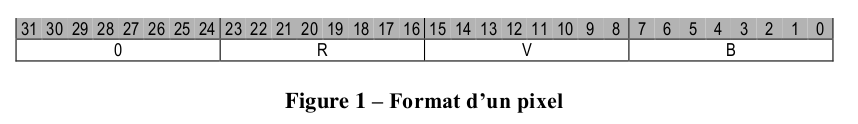
\includegraphics[width=\textwidth]{img/pixel.png}
   %\caption{Schéma RTL}
\end{figure}

\noindent Une image étant composée de lignes et colonnes de pixels, elle peut être vue ainsi :
\begin{figure}[!h]
   \centering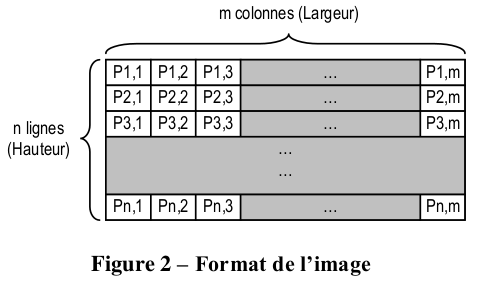
\includegraphics[height=6cm]{img/image_struct.png}
   %\caption{Schéma RTL}
\end{figure}

En mémoire, notre image sera représentée sous la forme d'un tableau d'entiers. Ce tableau de taille \textit{largeur * hauteur} contiendra bout à bout chaque ligne de l'image.

\section{Réalisation}
\subsection{Conversion niveau de gris}

On réalise le code assembleur de la conversion en niveau de gris. On effectuera une boucle parcourant chaque pixel et effectuant le calcul suivant :
\begin{figure}[!h]
   \centering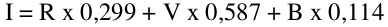
\includegraphics{img/formule.png}
   %\caption{Schéma RTL}
\end{figure}

Notre pixel en niveau de gris sera toujours stocké sur 32 bits, or on souhaite que la valeur du gris soit stocké dans l'octet de la composante bleue (les autres composantes seront à 0). Il convient donc de vérifier que notre calcul ne provoque pas de débordement (pas plus de 8 bits, soit la composante bleue).

\medskip

La somme des c\oe{}fficients que l'on applique à chaque composante est égale à 1 (0.299+0.587+0.114=1). Donc quelque soit les valeurs d'intensités des composantes, le résultat de conversion sera toujours inférieur ou égal à 255 (stocké sur 8 bits donc). \textbf{Il n'y a par conséquent aucun risque de débordement et notre composante de gris sera bien stockée sur 8 bits à la place de la composante bleue.}

\bigskip
Les calculs doivent être effectués en prenant en compte la virgule des coefficients.Les composantes de couleurs seront donc représentées sur 16 bits à virgule fixe avec un décalage de la virgule de +8.
Par exemple on écrira 42 ainsi :

\begin{center}
$\underbrace{
	\begin{tabular}{|c|c|c|c|c|c|c|c|}
	\hline
	0 & 0 & 1 & 0 & 1 & 0 & 1 & 0 \\
	\hline
	\end{tabular}}_{Partie\ entiere\ -\ Poids\ fort}$$\underbrace{
	\begin{tabular}{|c|c|c|c|c|c|c|c|}
	\hline
	0 & 0 & 0 & 0 & 0 & 0 & 0 & 0 \\
	\hline
	\end{tabular}}_{Partie\ decimale\ -\ Poids\ faible}$ 
\end{center}

Pour la partie décimale, il faut faire en sorte que celle-ci tienne sur 8 bits. On peut la décomposer sous la forme :
\begin{equation}
Partie\ decimale = 2^{-1} + 2^{-2} + 2^{-3} + 2^{-4} + 2^{-5} + 2^{-6} + 2^{-7} + 2^{-8}
\end{equation}
Soit : 
\begin{equation}
Partie\ decimale \times 256 = 2^{7} + 2^{6} + 2^{5} + 2^{4} + 2^{3} + 2^{2} + 2^{1} + 2^{0}
\end{equation}

Ce qui nous permet donc de représenter le nombre sur 8 bits. Cependant on effectue une petite erreur inévitable de l'ordre de $2^{-8}$ lorsque l'on décalera de 8 bits à nouveau, après les calculs.

\medskip

Après conversion et multiplication par 256 on trouve les valeurs héxadécimales arrondies suivantes :
\begin{center}
	\begin{tabular}{|l|c|c|}
		\hline
		Coef. du rouge & 0.299 & 0x4D \\
		\hline
		Coef. du vert & 0.587 & 0x96 \\
		\hline
		Coef. du bleu & 0.114 & 0x1D \\
		\hline
	\end{tabular}
\end{center}
Ces valeurs sont celles que l'on mettra dans la partie décimale des coefficients (la partie entière étant 0).

\medskip

Avant de produire le code assembleur, on s'intéresse au déroulement de la conversion d'un pixel en niveaux de gris. On prendra pour exemple le pixel suivant :
\begin{center}
    \begin{tabular}{|c|}
    \hline
    0 \\
    \hline
    \end{tabular}$\underbrace{
    \begin{tabular}{|c|}
    \hline
    127 \\
    \hline
    \end{tabular}}_{R}$$\underbrace{
    \begin{tabular}{|c|}
    \hline
    204\\
    \hline
    \end{tabular}}_{V}$$\underbrace{
    \begin{tabular}{|c|}
    \hline
    78 \\
    \hline
    \end{tabular}}_{B}$
\end{center}
On veut obtenir le niveau de gris dans la composante bleu.
On traite la composante bleue :
\begin{center}
$\underbrace{
    \begin{tabular}{|c|c|c|c|c|c|c|c|}
    \hline
    0 & 1 & 0 & 0 & 1 & 1 & 1 & 0 \\
    \hline
    \end{tabular}}_{78}$
    \begin{tabular}{|c|c|c|c|c|c|c|c|}
    \hline
    0 & 0 & 0 & 0 & 0 & 0 & 0 & 0 \\
    \hline
    \end{tabular}
\end{center}
$\times$\begin{center}
   \begin{tabular}{|c|c|c|c|c|c|c|c|}
    \hline
    0 & 0 & 0 & 0 & 0 & 0 & 0 & 0 \\
    \hline
    \end{tabular}$\underbrace{
    \begin{tabular}{|c|c|c|c|c|c|c|c|}
    \hline
    0 & 0 & 0 & 1 & 1 & 1 & 0 & 1\\
    \hline
    \end{tabular}}_{0x1D}$
\end{center}
$=$
\begin{center}
\begin{tabular}{|c||}
    \hline
    \textbf{0x00}\\
    \hline
    \end{tabular}$\underbrace{
    \begin{tabular}{|c|c|c|c|c|c|c|c|}
    \hline
    0 & 0 & 0 & 0 & 1 & 0 & 0 & 0 \\
    \hline
    \end{tabular}}_{Partie\ entiere\ =\ 8}$$\underbrace{
    \begin{tabular}{|c|c|c|c|c|c|c|c|}
    \hline
    1 & 1 & 0 & 1 & 0 & 1 & 1 & 0 \\
    \hline
    \end{tabular}}_{Partie\ decimale}$\begin{tabular}{||c|}
    \hline
    \textbf{0x00} \\
    \hline
    \end{tabular} 
\end{center}

Du fait de la multiplication entre 2 nombres de 16 bits, on a un résultat sur 32 bits avec une virgule décalée de 16 bits. Cependant on notera que les 8 bits de poids forts sont toujours à zéro (la partie entière du résultat est toujours inférieure à 255). De plus le résultat attendu en niveau de gris est un entier, donc la partie décimale sera ignorée dans le résultat final.

En répétant l'opération sur les composantes verte et rouge on obtient les 2 mots de 32 bits suivants :\\
\textbf{Rouge :}
\begin{center}
\begin{tabular}{|c||}
    \hline
    \textbf{0x00}\\
    \hline
    \end{tabular}$\underbrace{
    \begin{tabular}{|c|c|c|c|c|c|c|c|}
    \hline
    0 & 0 & 1 & 0 & 0 & 1 & 1 & 0 \\
    \hline
    \end{tabular}}_{Partie\ entiere\ =\ 38}$$\underbrace{
    \begin{tabular}{|c|c|c|c|c|c|c|c|}
    \hline
    0 & 0 & 1 & 1 & 0 & 0 & 1 & 1 \\
    \hline
    \end{tabular}}_{Partie\ decimale}$\begin{tabular}{||c|}
    \hline
    \textbf{0x00} \\
    \hline
    \end{tabular} 
\end{center}

\noindent \textbf{Vert :}
\begin{center}
\begin{tabular}{|c||}
    \hline
    \textbf{0x00}\\
    \hline
    \end{tabular}$\underbrace{
    \begin{tabular}{|c|c|c|c|c|c|c|c|}
    \hline
    0 & 1 & 1 & 1 & 0 & 1 & 1 & 1 \\
    \hline
    \end{tabular}}_{Partie\ entiere\ =\ 119}$$\underbrace{
    \begin{tabular}{|c|c|c|c|c|c|c|c|}
    \hline
    1 & 0 & 0 & 0 & 1 & 0 & 0 & 0 \\
    \hline
    \end{tabular}}_{Partie\ decimale}$\begin{tabular}{||c|}
    \hline
    \textbf{0x00} \\
    \hline
    \end{tabular} 
\end{center}

On souhaite maintenant obtenir un niveau de gris sur 8 bits. On additionne donc nos 3 résultats de 32 bits et on effectue un décalage de 16 bits à droite pour éliminer la partie décimale. On obtient donc :
\begin{center}
\begin{tabular}{|c||}
    \hline
    \textbf{0x00}\\
    \hline
    \end{tabular}$\underbrace{
    \begin{tabular}{|c|c|c|c|c|c|c|c|}
    \hline
    1 & 0 & 1 & 0 & 0 & 1 & 0 & 1 \\
    \hline
    \end{tabular}}_{Resultat\ =\ 165}$ 
\end{center}
On ne manipulera que les 8 bits de poids faible qui constituent le résultat. Ici on a 165 tandis que la valeur théorique du calcul donne 166,613. Il y a donc bien une erreur provoquée par la manipulation utilisée pour considérer les parties décimales. Cependant l'\oe{}il humain ne différencie gère plus que 50 intensités différentes, et compte tenu de notre faible erreur, ceci n'est à priori pas visible à l'\oe{}il nu.

\subsection{Code assembleur}
On réalise ensuite notre programme en assembleur. \textbf{Dans les faits, nous manipulons les composantes de couleur sur 8 bits ainsi que les c\oe{}fficients de multiplication sur 8 bits, par conséquent nous obtenons un résultat de multiplication sur 16 bits, et nous ne conservons que les 8 bits de poids fort.}

\assembly
\begin{lstlisting}
; CODE FOURNI
; ...

    ;*****************************************************************
    ;*****************************************************************
    ; Ajoutez votre code ici
    ;*****************************************************************
    ;*****************************************************************
    
    dec ecx
    imul ecx,4

boucle: 
    movzx ebx, byte ptr [esi+ecx] ; on stocke la valeur du bleu
    imul ebx, 29d ; 29 = 0.114*256
    mov eax,ebx

    movzx ebx, byte ptr [esi+ecx+1] ; on stocke la valeur du vert
    imul ebx, 150d ; 150 = 0.587*256
    add eax,ebx

    movzx ebx, byte ptr [esi+ecx+2] ; on stocke la valeur du rouge
    imul ebx, 77d ; 77 = 0.299*256
    add eax,ebx
    shr eax, 8 ; décalage de 8 bits pour ne conserver que la partie entière

    mov [edi+ecx], eax ; on sauvegarde la valeur du pixel que l'on copie dans l'image de destination

    sub ecx,4
    jne boucle
fin:

; ...
; CODE FOURNI
\end{lstlisting}

On test le programme en C et en assembleur et on obtient les temps suivants (à gauche en C et à droite en assembleur ):
\begin{figure}[!h]
   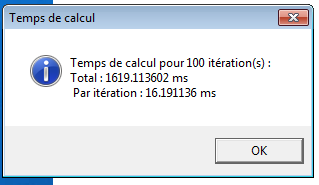
\includegraphics[width=0.5\textwidth]{img/gris_c.png}
   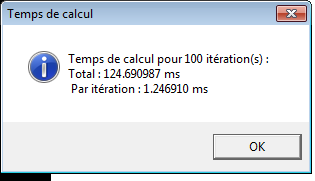
\includegraphics[width=0.5\textwidth]{img/gris_assembly.png}
   \caption{Temps conversion niveaux de gris}
\end{figure}

On constate donc une très grande différence de temps d'execution. Notre code assembleur est 10 fois plus rapide que la fonction C. Il est fonctionnel (comparaison visuelle avec le traitement en C).

\medskip

Pour obtenir une image en vrai noir et blanc (et non uniquement sur la composante bleue comme dans le sujet), il suffit de rajouter ce bout de code à la fin de notre code, qui copie la valeur du gris dans les composantes rouge et verte :
\begin{lstlisting}
; ...
shr eax,8

; VRAI NOIR ET BLANC
mov ah,al
shl eax,8
mov al,ah

mov [edi+ecx], eax
; ...
\end{lstlisting}
Le résultat que l'on obtient est le suivant :
\begin{figure}[!h]
   \centering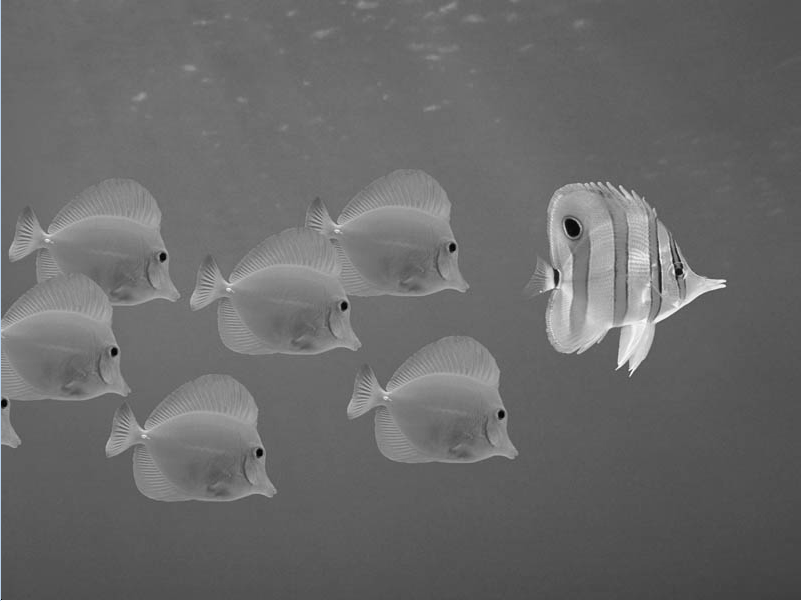
\includegraphics[width=\textwidth]{img/niveaux_gris.png}
   \caption{Image en niveaux de gris}
\end{figure}
\\
Nous pouvons donc passer à la partie suivante, à savoir la détection des contours dans l'image.

\chapter{Détection des contours}
\section{Présentation}
La détection des contours au sein d'une image est un traitement d'image assez classique, très utile pour la détection/reconnaissance d'objets par exemple.

\subsection{Principe de détection}
Les zones de contours sont caractérisées par un fort contraste. La détection de contours se réduit donc à la détection des zones à fort contraste. Pour se faire il y a 2 grands types de méthodes : l'analyse du laplacien de l'image et l'analyse du gradient. L'analyse du gradient sera implémentée ici.

\medskip

On utilisera l'opérateur de Sobel qui permet une mesure, en deux dimensions, du gradient de l'intensité d'une image en niveaux de gris. Cet opérateur se présente sous la forme de 2 masques de convolution $S_x$ et $S_y$ qui fournissent le gradient de chaque pixel (respectivement dans les directions \textit{x} et \textit{y}).\\
\begin{center}
$ G_x=
 \begin{bmatrix}
    -1 & 0 & 1 \\
    -2 & 0 & 2 \\
    -1 & 0 & 1
 \end{bmatrix}$
 et 
$G_y=
 \begin{bmatrix}
    1 & 2 & 1 \\
    0 & 0 & 0 \\
    -1 & -2 & -1
 \end{bmatrix}$
\end{center} 
La norme $G$ du gradient est calculée comme suit :
\begin{equation}
|G| = \sqrt{G_x^2 + G_y^2}    
\end{equation}
Mais pour faciliter les calculs on nous propose de simplifier comme suit :
\begin{equation}
|G| = |G_x| + |G_y|    
\end{equation}
\\
Le gradient de chaque pixel sera donc calculé en appliquant chaque masque sur chaque pixel, ligne par ligne. Un exemple nous est proposé :
\begin{figure}[!h]
   \centering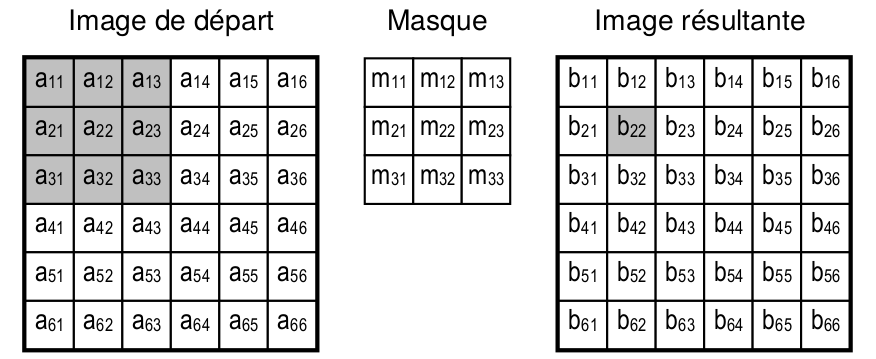
\includegraphics[height=5cm]{img/exemple_masque.png}
   \caption{Applicaton du masque}
\end{figure}
\\
Ici la valeur du pixel $b_{22}$ est :
\begin{equation}
b_{22} = m_{11}a_{11} + m_{12}a_{12} + m_{13}a_{13} + m_{21}a_{21} + m_{22}a_{22} + m_{23}a_{23} + m_{31}a_{31} + m_{32}a_{32} + m_{33}a_{33}     
\end{equation}
Evidemment les lignes et colonnes en bordure de l'image ne pourront pas être traitées par un masque de dimension 3x3, les pixels correspondant ne seront donc pas pris en compte (ils seront laissés noirs).

\subsection{Algorithme de traitement}
On va donc parcourir tout les pixels de l'image source pour calculer le gradient et le mettre dans le pixel correspondant de l'image de destination :
\begin{enumerate}
\item On applique $G_x$ et $G_y$
\item On somme leurs valeurs absolues
\item On veut afficher l'image en noir sur fond blanc donc on "inverse" les pixels en faisant $255-G$
\item Si la valeur est négative alors on met le pixel à 0
\item On stocke la valeur dans le pixel de l'image de destination
\end{enumerate}

\section{Réalisation}
On va donc réaliser notre fonction de traitement. On considère que le niveau de gris de chaque pixel se trouve dans la composante bleue de celui-ci. On utilisera les registres de la manière ci-dessous :
\begin{itemize}
    \item \textbf{ESI} : Adresse du premier pixel (de la matrice) source
    \item \textbf{EDI} : Adresse du pixel de destination
    \item \textbf{EBP} : Taille d'une ligne en pixel (sauvegarde du pointeur de pile avant cela)
    \item \textbf{ECX} : Poids forts (16 bits) = compteur de lignes restantes = nombre de lignes - 2\\Poids faibles (16 bits) = compteur de colonnes restantes = nombre de colonnes - 2
    \item \textbf{EBX} : Valeur de $G_x$
    \item \textbf{EDX} : Valeur de $G_y$
\end{itemize}
Pour respecter cette organisation on initialise les registres servant à enregistrer les adresses sources et destination :

\begin{lstlisting}[language={[x86masm]Assembler}]
mov     esi, [ebp + 20]
mov     edi, [ebp + 24]
\end{lstlisting}
On initialisera \lstinline{ebp} à \lstinline{[EBP+8]} (la longueur d'une ligne) uniquement après avoir initialisé les autres registres. En effet \lstinline{ebp} nous sert aussi de sauvegarde du pointeur de pile et est nécessaire pour récupérer les différents paramètres.

\subsection{Double itération}
Comme indiqué précèdement, le registre \lstinline{ecx} sera utilisé en tant que double compteur. Les poids forts (16 bits) compteront les lignes restantes à traiter et les poids faibles les colonnes restantes à traiter.

\subsubsection{Itération sur les lignes}
On initialise les poids forts ainsi :
\begin{lstlisting}[language={[x86masm]Assembler}]
mov ecx, [ebp + 12]  ; On déplace le nombre de ligne dans ecx
sub     ecx, 2 ; On soustrait de 2 (suppresion des bords)
shl     ecx,16 ; On décale la valeur sur les 16 bits de poids forts
\end{lstlisting}

En fin de boucle on décrémente les bits de poids forts et on vérifie que ce n'est pas fini, sinon on reboucle :
\begin{lstlisting}[language={[x86masm]Assembler}]
sub ecx, 65536 ; decremente de 1 les 16 bits de poids fort
cmp ecx,0 ; On compare avec zéro
jne traitement_ligne ; Si ce n'est pas égal à zéro on lance un nouveau traitement de ligne
\end{lstlisting}

À la fin du traitement d'une ligne \lstinline{edi} et \lstinline{esi} doivent avancer de deux pixels d'un coup pour passer à la ligne suivante et sauter la dernière colonne et la première colonne de pixels.

\subsubsection{Itération sur les colonnes}
Pour les colonnes on utilisera les 16 bits de poids faibles de \lstinline{ecx} soit le registre \lstinline{cx}. Au début d'une boucle sur une ligne on l'initialise au nombre de colonnes à traiter, soit la longueur d'une ligne (valeur stockée dans \lstinline{ebp}) en enlevant 2 colonnes (la première et la dernière).\\
Dans cette boucle, après avoir traité un pixel, on passe au pixel suivant. On avance donc \lstinline{edi} et \lstinline{esi} d'un pixel soit 4 octets.

\subsubsection{Implémentation de la boucle}

On obtient donc notre structure de boucle suivante :
\begin{lstlisting}[language={[x86masm]Assembler}]
; ****** Détection de contours - boucle itérative ******
mov     esi, [ebp + 20] ; tmp1
mov     edi, [ebp + 24] ; tmp2

; On stocke le nombre de lignes à traiter dans les bits de poids fort de ECX (hauteur)
mov ecx, [ebp + 12]
sub     ecx, 2
shl     ecx, 16

mov ebp, [ebp + 8] ; on stocke la longueur d'une ligne = le nombre de colonnes = largeur
; On saute la première ligne et on passe à la deuxième case (+4)

lea edi, [edi+ebp*4+4]

traitement_ligne:
add ecx, ebp ; nombre de colonnes à traiter
sub cx, 2

    traitement_colonne:
    
    ; ****************************
    ; Traitement pixel ici
    ;*****************************

    ; Après avoir traité le pixel, on avance d'un pixel
    add edi, 4
    add esi, 4
    dec cx ; on décremente le nombre de colonnes à traiter
    cmp cx, 0
    jne traitement_colonne

; Passage à la deuxième case de la ligne suivante
add edi, 8
add esi, 8

sub ecx, 65536 ; decremente de 1 les 16 bits de poids fort <=> decremente compteur de lignes
cmp ecx,0
jne traitement_ligne
\end{lstlisting}

\section{Calcul du gradient}
\subsection{Implémentation}
Il faut maintenant programmer le coeur de l'application : le traitement du pixel. On stockera $G_x$ dans \lstinline{ebx} et $G_y$ dans \lstinline{edx}.
\paragraph{}
Si le registre \lstinline{esi} contient l'adresse de $a_{11}$ de l'image source (et que \lstinline{ebp} contient la longueur d'une  ligne), alors l'adresse de :

\begin{itemize}
    \item $a_{12}$ : \lstinline{[esi + 4]} => On avance d'un pixel (4 octets) 
    \item $a_{21}$ : \lstinline{[esi + ebp*4]} => On avance d'une ligne (longueur ligne en pixels*4)
    \item $a_{31}$ : \lstinline{[esi + ebp*8]} => On avance de 2 lignes (2*longueur ligne*4) 
\end{itemize}

\bigskip

Pour effectuer le calcul de $G_x$ et $G_y$ sur un pixel on multipliera l'intensité de chaque pixel par l'élément correspondant de la matrice puis on sommera les différents résultats.
Par exemple pour $G_x$ :
\assembly
\begin{lstlisting}
mov ebx, [esi]
mov eax, [esi+ebp*4]
imul eax, 2
add ebx, eax
add ebx, [esi+ebp*8] ; on saute 2 lignes
neg ebx
add ebx, [esi+8]
mov eax, [esi+8+ebp*4]
imul eax, 2
add ebx, eax
add ebx, [esi+8+ebp*8]
\end{lstlisting}
Le principe est le même pour le calcul de $G_y$, seuls les c\oe{}fficients changent.

\bigskip

Après le calcul des coefficients, il est nécessaire de récupérer la valeur absolue. Pour $G_x$ on obtient :
\begin{lstlisting}
add ebx, [esi+8+ebp*8] ; Dernière opération arithmétique du calcul de Gx
jns pasneg ; Si le résultat n'est pas négatif on saute la prochaine instruction
neg ebx ; Sinon on change le signe (on le rend donc positif)
pasneg:
; Suite du programme
\end{lstlisting}

\bigskip

On somme ensuite les 2 composantes et on effectue la fin de l'algorithme : normalisation par rapport à 255 et affichage en niveaux de gris \og négatif\fg{} (bordure noir sur fond blanc).\\
On utilise le code ci-dessous :
\begin{lstlisting}
add ebx, edx ; On additionne les 2 composantes

neg ebx
add ebx,255 ; ebx = 255-ebx
cmp ebx,0
jg endd
mov ebx,0

endd:
mov eax,ebx
shl eax,8 ; Via plusieurs décalage, on met la valeur du gradient dans chaque composante du pixel
add ebx,eax
shl eax,8
add ebx,eax
mov [edi], ebx ; On met le pixel dans l'image de destination
\end{lstlisting}

\subsection{Résultat}
On teste donc le code complet (disponible en Annexe) et on obtient le bon résultat (voir figure ci-dessous).

\medskip

On détecte correctement les contours de l'image et on affiche bien le résultat en contours noirs sur fond blanc. On compare les temps d'execution (en C à gauche en assembleur à droite) sur la figure ci-dessous.

\medskip

On constate que notre code assembleur est bien plus rapide que le traitement en C. Pour 100 itérations on gagne une seconde de traitement.

\begin{figure}[!h]
   \centering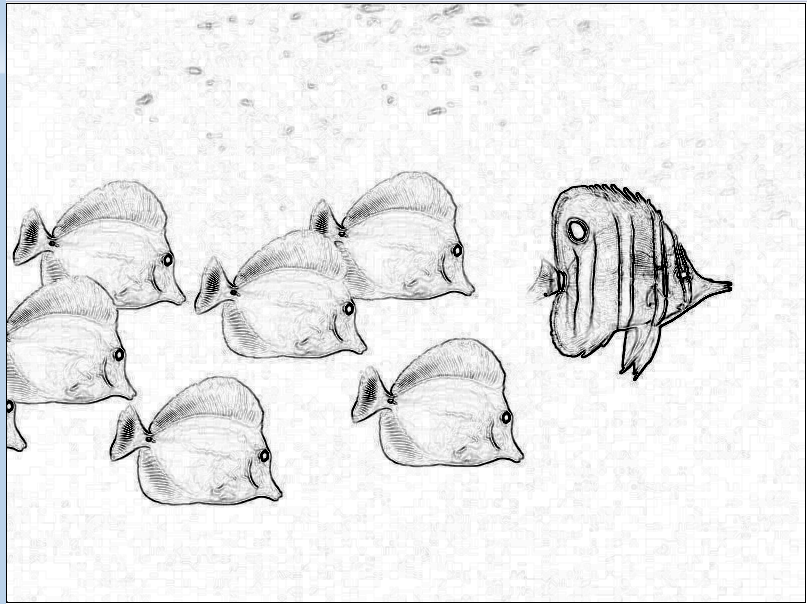
\includegraphics[width=\textwidth]{img/contours.png}
   \caption{Détection des contours}
\end{figure}

\begin{figure}[!h]
   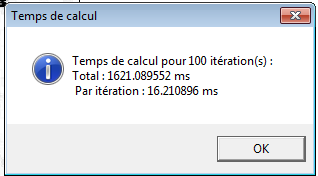
\includegraphics[width=0.5\textwidth]{img/contours_c.png}
   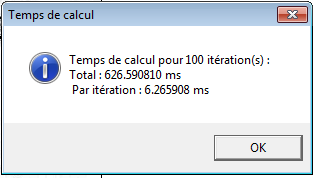
\includegraphics[width=0.5\textwidth]{img/contours_assembly.png}
   \caption{Temps de détection totale des contours}
\end{figure}
\chapter{Conclusion générale}

\section{OpenGL ou Unity}

La plus grosse problématique du projet aura été le choix entre Unity et OpenGL. Nous étions initalement partis sur du développement en OpenGL mais heureusement, en début d'année 2015, Unity a rendu son moteur totalement gratuit, nous permettant ainsi de pouvoir l'utiliser. Nous nous en sommes rendus compte peu de temps après le début du projet et avons ainsi changé de technologie. Nous avons tout de même eu le temps d'essayer OpenGL et il s'était avéré que le développement aurait été bien trop dur et presque impossible. Effectivement, nous ne connaissions pas cette technologie et la contrainte de temps (un semestre) ne nous aurait pas permis de l'appréhender.

\section{Problèmes}

Un autre problème aura été l'utilisation du SDK de Google. Au départ nous ne savions pas comment faire déplacer le joueur, nous étions donc partis sur l'utilisation d'une \textit{library} tierce, Dive. Or il s'est avéré que cette \textit{library} souffrait d'un bug au niveau du gyroscope. Nous avons finalalement réussi à utiliser uniquement le SDK de Google et faire avancer notre joueur.

\section{Jeu final et objectifs}

Au final, un seul de nos objectifs complémentaires a été atteint : rajouter une ambiance sonore (une musique de fond). Nous sommes néanmoins très satisfaits du résultat visuel et du jeu de manière générale. Avoir plus de temps nous aurait probablement permis d'atteindre d'autres objectifs.

\end{document}
